\documentclass[12pt]{article}%
\usepackage[T1]{fontenc}
\usepackage[toc,page]{appendix}
\usepackage[latin9]{inputenc}
\usepackage{pdfsync}
\usepackage{geometry}
\usepackage{enumerate}
\geometry{verbose,tmargin=2cm,bmargin=2cm,lmargin=2cm,rmargin=2cm}
\usepackage{amstext}
\usepackage{amssymb,amsmath}
\usepackage{esint}
\usepackage{amsthm}
\theoremstyle{plain}
\usepackage{graphicx}
\numberwithin{equation}{section}
\usepackage{indentfirst}
\usepackage{algorithm}
\usepackage{algorithmic}
\newtheorem{thm}{Theorem}[section]
\newtheorem{lem}{Lemma}[section]
\newtheorem{prop}[thm]{Proposition}
\newtheorem{col}{Corollary}[section]
\newtheorem{dfn}{Definition}[section]
\newtheorem{conj}{Conjecture}[section]
\newtheorem{exmp}{Example}[section]
\newtheorem{remark}{Remark}
\newcommand{\Q}{\mathbb{Q}}
\newcommand{\R}{\mathbb{R}}
\newcommand{\C}{\mathbb{C}}
\newcommand{\Z}{\mathbb{Z}}
\newcommand{\BEA}{\begin{eqnarray}}
\newcommand{\EEA}{\end{eqnarray}}
\usepackage{hyperref}
\setcounter{secnumdepth}{5}
\hypersetup{bookmarksopen=true}
\usepackage{mathrsfs}
\usepackage{float}
\usepackage{subcaption}
\usepackage{color}
\begin{document}

\title{Notes on Laplacian on domains with fractal boundary}
\author{Qile Yan}
\date{\today}
\maketitle
\section{Problem setting } 
\subsection{fractal boundary with a few steps of Koch snowflake}
  \begin{figure}[H]%
    \centering
         \begin{subfigure}[h]{0.45\linewidth}
         \caption{$n=2$}
\includegraphics[width=\linewidth]{figures/Ex1/Ex1_snow_n2.pdf}
\end{subfigure}
 \begin{subfigure}[h]{0.45\linewidth}
 \caption{$n=4$}
\includegraphics[width=\linewidth]{figures/Ex1/Ex1_snow_n4.pdf}
\end{subfigure}
  \caption{Unit square with the top edge replaced by a Koch snowflake with $n$ iterations.}
  \label{fig:snow_2d}
 \end{figure}
2D: Let $n$ be the number of iterations in the snowflake (See Fig. \ref{fig:snow_2d}, meshsize=0.02 for all vertices in .geo).  The total number of small sides is $4^n$ and the small length scale $l=\left(\frac{1}{3}\right)^n$. Thus, the perimeter of the snowflake $L_p=\left(\frac{4}{3}\right)^n$. 

Python script for creating the 2D mesh: snow\_square.py. 

3D: Let $n$ be the number of iterations in the snowflake (See Fig. \ref{fig:snow_3d}, meshsize=0.1 for all vertices in .geo). The total number of small squares is $13^n$ and the small area is $l=(\frac{1}{9})^n$. Thus, the perimeter of the snowflake $L_p=\left(\frac{13}{9}\right)^n$. 

%Remark: In Fig. \ref{fig:snow_3d}(c), the figure is created by Matlab as following: convert .msh file to .stl file in gmsh then it is converted to .obj file in MeshLab. If we plot the mesh using firedrake directly, the top surface has the same color which make it hard to read.

Python script for creating the 3D mesh: snow\_cube.py. 

  \begin{figure}[H]%
    \centering
         \begin{subfigure}[h]{0.45\linewidth}
         \caption{$n=2$}
\includegraphics[width=\linewidth]{figures/Ex2/Ex2_snow_cube_2.png}
\end{subfigure}
% \begin{subfigure}[h]{0.32\linewidth}
 %\caption{$n=2$}
%\includegraphics[width=\linewidth]{snow_cube_2.png}
%\end{subfigure}
 \begin{subfigure}[h]{0.45\linewidth}
 \caption{$n=3$}
\includegraphics[width=\linewidth]{figures/Ex2/Ex2_snow_cube_3.png}
\end{subfigure}
  \caption{Unit cube with the top surface replaced by a Koch snowflake with $n$ iterations.}
  \label{fig:snow_3d}
 \end{figure}


\subsection{PDEs}
Solve 
\begin{equation}
-\text{div}(D\text{grad}u)=0\quad\text{on}\ \Omega
\label{eq1}
\end{equation}
$\Omega$:
\begin{enumerate}[(a)]
\item the unit square in which the top edge has been replaced by a prefractal.
\item the unit cube in which the top face is replaced by a prefractal.
\end{enumerate}
Boundary conditions: 
\begin{enumerate}[(a)]
\item on bottom edge, Dirichlet: $u=1$.
\item on sides, homogeneous Neumann: $\frac{\partial u}{\partial n}=0$.
\item on prefractal top edge, Robin boundary conditions: $\Lambda\frac{\partial u}{\partial n}+u=0$.
\end{enumerate}

The total flux through the top edge: 
$$
\Phi:=\int_{top}-D\frac{\partial u}{\partial n}d\sigma=\frac{D}{\Lambda}\int_{top}ud\sigma.
$$
We need to see how $\Phi$ depends on $\Lambda$ for $0\leq \Lambda\leq 2L_p$.

\section{Test firedrake solver on 2D and 3D}
Consider the Laplace equation $-\text{div}(D\text{grad}u)=f$ with non homogeneous condition: 
\begin{enumerate}[(a)]
\item on bottom edge/surface, Dirichlet: $u=g$.
\item on sides, homogeneous Neumann: $\frac{\partial u}{\partial n}=k$.
\item on prefractal top edge/surface, Robin boundary conditions: $\Lambda\frac{\partial u}{\partial n}+u=l$.
\end{enumerate}

The weak formulation: Find $u\in H^1$ with $u=g$ on bottom such that 
$$
\int_\Omega D\text{grad}(u)\cdot \text{grad}(v) dx+\int_{top}\frac{D}{\Lambda}u vds=\int_\Omega fv dx+\int_{top}\frac{1}{\Lambda} lvds+\int_{sides}kvds,\quad \forall v\in H^1_0
$$
\subsection{2D case}
In Fig. \ref{fig:Ex1_test}, we plot the error in $L^2$ and $H^1$ norm with respect to mesh size $h$. The manufactured solution is $u(x,y)= 2+x^2+y$ on the unit square with snowflake ($n=4$ iterations). The Lagrange linear element is used. The uniform refinement is done by built-in function MeshHierarchy.

The test python script on 2D is: test-robin-solver.py. 

\begin{figure}[H]%
    \centering
         \begin{subfigure}[h]{0.45\linewidth}
          \caption{Error vs mesh size}
\includegraphics[width=\linewidth]{figures/Ex1/Ex1_test.png}
\end{subfigure}
  \begin{subfigure}[h]{0.45\linewidth}
   \caption{Error vs degree of freedom}
\includegraphics[width=\linewidth]{figures/Ex1/Ex1_test_dof.png}
\end{subfigure}
  \caption{Unit square: Solution $u=x^2+y+2$.}
  \label{fig:Ex1_test}
 \end{figure}

\subsection{3D case}
In Fig. \ref{fig:Ex2_test} and Fig.  \ref{fig:Ex2_test_2}, we plot the error in $L^2$ and $H^1$ norm with respect to mesh size $h$ and degree of freedom where domain is unit cube with snowflake $n=3$ iterations. Here, we use the standard Lagrange linear element is used. To check the convergence rate, the uniform refinement is done by built-in function MeshHierarchy on the mesh in Fig. \ref{fig:snow_3d} (b). We consider two manufactured solutions (a).  $u(x,y,z)= 2+x+3y+z$.  (b). $u(x,y,z)= 2+x^2+3xy+yz$. The first one is a linear function in the element space while the second one is not.

 In Fig. \ref{fig:Ex2_test}, the discrete linear system is solved by computing LU factorisation. In the code, we set " solver\_parameters={'ksp\_type': 'preonly', 'pc\_type': 'lu'}) "
 
 In Fig. \ref{fig:Ex2_test_2}, the linear system is solved using Krylov subspace methods (conjugate gradient method since the operator is SPD). Besides, the preconditioner is chosen to be BoomerAMG. In the code, we set "solver\_parameters={'ksp\_type': 'cg', 'pc\_type': 'hypre','pc\_hypre\_type': 'boomeramg'} ".

From the first row of Fig. \ref{fig:Ex2_test} and Fig. \ref{fig:Ex2_test_2}, we can see that for linear solution $u$ the only round off error appears in the case when LU factorisation is used. But the error from using Krylov subspace is around $5*10^{-7}$ to  $5*10^{-6}$. On the other hand, the Krylov subspace method solve the linear system faster and also could deal with a finer mesh when degree of freedom is $10^7$.

The test python script on 3D is: test-robin-solver-cube.py.  The script is run by the following parallelsim command 

mpiexec -n 16 python test-robin-solver-cube.py


\begin{figure}[H]%
    \centering
         \begin{subfigure}[h]{0.45\linewidth}
          \caption{Error vs mesh size}
\includegraphics[width=\linewidth]{figures/Ex2/Ex2_test_LU.png}
\end{subfigure}
    \begin{subfigure}[h]{0.45\linewidth}
     \caption{Error vs degree of freedom}
\includegraphics[width=\linewidth]{figures/Ex2/Ex2_test_dof_LU.png}
\end{subfigure}
  \begin{subfigure}[h]{0.45\linewidth}
          \caption{Error vs mesh size}
\includegraphics[width=\linewidth]{figures/Ex2/Ex2_test_2_LU.png}
\end{subfigure}
    \begin{subfigure}[h]{0.45\linewidth}
     \caption{Error vs degree of freedom}
\includegraphics[width=\linewidth]{figures/Ex2/Ex2_test_2_dof_LU.png}
\end{subfigure}
  \caption{Unit cube: The linear system is solved by  LU factorisation. }
  \label{fig:Ex2_test}
 \end{figure}
\begin{figure}[H]%
    \centering
         \begin{subfigure}[h]{0.45\linewidth}
          \caption{Error vs mesh size}
\includegraphics[width=\linewidth]{figures/Ex2/Ex2_test.png}
\end{subfigure}
    \begin{subfigure}[h]{0.45\linewidth}
     \caption{Error vs degree of freedom}
\includegraphics[width=\linewidth]{figures/Ex2/Ex2_test_dof.png}
\end{subfigure}
  \begin{subfigure}[h]{0.45\linewidth}
          \caption{Error vs mesh size}
\includegraphics[width=\linewidth]{figures/Ex2/Ex2_test_2.png}
\end{subfigure}
    \begin{subfigure}[h]{0.45\linewidth}
     \caption{Error vs degree of freedom}
\includegraphics[width=\linewidth]{figures/Ex2/Ex2_test_2_dof.png}
\end{subfigure}
  \caption{Unit cube. The linear system is solved by Krylov subspace methods }
  \label{fig:Ex2_test_2}
 \end{figure}



\section{$\Omega$ is unit square and D is constant}
Now, we solve the PDE (\ref{eq1}) on 2D unit square using firedrake with the finest mesh in Fig. \ref{fig:test_on_2d}. In Fig. \ref{flux_square}, we plot the flux $\Phi=\int_{top}-D\frac{\partial u}{\partial n}d\sigma$ with different choice of $\Lambda$.
  \begin{figure}[H]%
    \centering
         \begin{subfigure}[h]{0.45\linewidth}
         \caption{Solution when $D=1,\Lambda=1$}
\includegraphics[width=\linewidth]{figures/Ex1/solution_D1_Lam1.png}
\end{subfigure}
 \begin{subfigure}[h]{0.45\linewidth}
         \caption{Total flux vs $\Lambda$}
\includegraphics[width=\linewidth]{figures/Ex1/Phi_Lam_n4.png}
\end{subfigure}
  \caption{Snowflake with $n=4$ iterations. (a). Solutions. (b) Total flux vs $\Lambda$ when $D=1$. Python script: main\_flux.py.}
  \label{flux_square}
 \end{figure}

\section{$\Omega$ is unit cube and D is constant}
Now, we solve the PDE (\ref{eq1}) on 3D unit cube using firedrake with the finest mesh in Fig. \ref{fig:test_on_3d_2}. In Fig. \ref{flux_cube}, we plot the flux $\Phi=\int_{top}-D\frac{\partial u}{\partial n}d\sigma$ with different choice of $\Lambda$.
  \begin{figure}[H]%
    \centering
 \begin{subfigure}[h]{0.45\linewidth}
         \caption{Total flux vs $\Lambda$}
\includegraphics[width=\linewidth]{figures/Ex2/Phi_Lam_cube.png}
\end{subfigure}
  \caption{Snowflake with $n=3$ iterations on Cube. Total flux vs $\Lambda$ when $D=1$. Python script: main\_flux.py.}
  \label{flux_cube}
 \end{figure}



\section{Fractal harmonic measure}

\subsection{Result on unit disk} 
In this section, we consider the domain $\Omega$ is a unit disk (see Fig. \ref{fig:unit_disk}).
  \begin{figure}[H]%
    \centering
         \begin{subfigure}[h]{0.45\linewidth}
  \includegraphics[width=\linewidth]{figures/Ex3/unit_disk.pdf}
\end{subfigure}
  \caption{Unit disk.}
  \label{fig:unit_disk}
 \end{figure}

We first test the firedrake solver on the PDE:
\begin{equation}
-\Delta u =f \quad\text{on }\Omega
\end{equation}
with $u=g$ on $\partial \Omega$. 

In Fig. \ref{fig:Ex3_disk_test} and Fig.  \ref{fig:Ex3_disk_test_2}, we plot the error in $L^2$ and $H^1$ norm with respect to mesh size $h$ and degree of freedom. \ref{fig:Ex3_disk_test}, the manufactured solution is $u(x,y)= 2+x+3y$. In Fig. \ref{fig:Ex3_disk_test_2}, the manufactured solution is $u(x,y,z)= 2+x^2+y$. The Lagrange linear element is used. The uniform refinement is done by built-in function MeshHierarchy.

\begin{figure}[H]%
    \centering
         \begin{subfigure}[h]{0.45\linewidth}
          \caption{Error vs mesh size}
\includegraphics[width=\linewidth]{figures/Ex3/disk_test1.png}
\end{subfigure}
  \begin{subfigure}[h]{0.45\linewidth}
   \caption{Error vs degree of freedom}
\includegraphics[width=\linewidth]{figures/Ex3/disk_test1_dof.png}
\end{subfigure}
  \caption{Unit disk: manufactured solution $u=x+3y+2$. Note that only round off error appears here since the solution is in the linear finite element space.  Remark: Here, we use the Krylov subspace method with BoomerAMG in preconditioner in the solver. If we change the solver to be LU factorisation, the error here would be around $10^{-14}\sim~10^{-15}$.}
  \label{fig:Ex3_disk_test}
 \end{figure}
 \begin{figure}[H]%
    \centering
         \begin{subfigure}[h]{0.45\linewidth}
          \caption{Error vs mesh size}
\includegraphics[width=\linewidth]{figures/Ex3/disk_test2.png}
\end{subfigure}
  \begin{subfigure}[h]{0.45\linewidth}
   \caption{Error vs degree of freedom}
\includegraphics[width=\linewidth]{figures/Ex3/disk_test2_dof.png}
\end{subfigure}
  \caption{Unit disk: manufactured solution $u=x^2+y+2$.}
  \label{fig:Ex3_disk_test_2}
 \end{figure}
 
 Next, we solve the PDE 
\begin{equation}
-\Delta u =f \quad\text{on }\Omega
\label{eqn:unit_disk}
\end{equation}
with $u=0$ on the unit disk and evaluate the solution at points from center to boundary.  In particular, we evaluate the solutions at
 \begin{equation}
 \textbf{x}_i=(0,1-1/2^i),\quad 0\leq i\leq n_{max}.
 \label{eqn:unit_disk_seq}
 \end{equation}

 In Fig. \ref{Ex3_disk_solution}, we show the results of the PDE (\ref{eqn:unit_disk}) with a different $f$. That is, we define $f$ as 
 $$
 f(x,y)=e^{-4((x-0.5)^2+(y-0.5)^2)}.
 $$
  \begin{figure}[H]%
    \centering
         \begin{subfigure}[h]{0.45\linewidth}
         \caption{f}
\includegraphics[width=\linewidth]{figures/Ex3/Ex3_disk_f.png}
\end{subfigure}
 \begin{subfigure}[h]{0.45\linewidth}
         \caption{Solution $u$}
\includegraphics[width=\linewidth]{figures/Ex3/Ex3_disk_solution.png}
\end{subfigure}
\\
\begin{subfigure}[h]{0.45\linewidth}
\caption{Evaluation at $\{\textbf{x}_i\}_{i=0}^4$.}
\includegraphics[width=\linewidth]{figures/Ex3/Ex3_disk_evaluate.png}
\end{subfigure}
\begin{subfigure}[h]{0.45\linewidth}
\caption{Evaluation at $\{\textbf{x}_i\}_{i=0}^4$. loglog plot}
\includegraphics[width=\linewidth]{figures/Ex3/Ex3_disk_evaluate_log.png}
\end{subfigure}
  \caption{On unit disk.   (a). force term $f$. (b) solution $u$. (c). Evaluation of solution at a sequence points $\{\textbf{x}_i\}_{i=0}^{10}$ where $\textbf{x}_i$ is defined as in (\ref{eqn:unit_disk_seq}). (d). loglog plot}
  \label{Ex3_disk_solution}
 \end{figure}
   
\subsection{On snowflake boundary domain}
In this note we solve the PDE 
\begin{equation}
-\Delta u =f \quad\text{on }\Omega
\label{eqn:Ex3}
\end{equation}
with $u=0$ on $\partial \Omega$. Here, $\Omega$ is a unit square where each edges are replaced by the Koch snowflake (See Fig. \ref{fig:snow_2d_Dirichlet}). In this note, we use the FEM python package firedrake solving the PDE. 

  \begin{figure}[H]%
    \centering
         \begin{subfigure}[h]{0.45\linewidth}
         \caption{$n=2$}
\includegraphics[width=\linewidth]{figures/Ex3/Ex3_snow_square_2.pdf}
\end{subfigure}
 \begin{subfigure}[h]{0.45\linewidth}
 \caption{$n=4$}
\includegraphics[width=\linewidth]{figures/Ex3/Ex3_snow_square_4.pdf}
\end{subfigure}
  \caption{Unit square with each edges replaced by a Koch snowflake with $n$ iterations. Meshsize is 0.5 for each vertices in .geo file.}
  \label{fig:snow_2d_Dirichlet}
 \end{figure}

In Fig. \ref{fig:Ex3_test} and Fig.  \ref{fig:Ex3_test_2}, we plot the error in $L^2$ and $H^1$ norm with respect to mesh size $h$ and degree of freedom where domain is unit square with snowflake ($n=4$ iterations). In Fig. \ref{fig:Ex3_test}, the manufactured solution is $u(x,y)= 2+x+3y$. In Fig. \ref{fig:Ex3_test_2}, the manufactured solution is $u(x,y,z)= 2+x^2+y$. The Lagrange linear element is used. The uniform refinement is done by built-in function MeshHierarchy.

\begin{figure}[H]%
    \centering
         \begin{subfigure}[h]{0.45\linewidth}
          \caption{Error vs mesh size}
\includegraphics[width=\linewidth]{figures/Ex3/Ex3_test1.png}
\end{subfigure}
  \begin{subfigure}[h]{0.45\linewidth}
   \caption{Error vs degree of freedom}
\includegraphics[width=\linewidth]{figures/Ex3/Ex3_test1_dof.png}
\end{subfigure}
  \caption{Unit square: manufactured solution $u=x+3y+2$. Note that only round off error appears here since the solution is in the linear finite element space.}
  \label{fig:Ex3_test}
 \end{figure}
 \begin{figure}[H]%
    \centering
         \begin{subfigure}[h]{0.45\linewidth}
          \caption{Error vs mesh size}
\includegraphics[width=\linewidth]{figures/Ex3/Ex3_test2.png}
\end{subfigure}
  \begin{subfigure}[h]{0.45\linewidth}
   \caption{Error vs degree of freedom}
\includegraphics[width=\linewidth]{figures/Ex3/Ex3_test2_dof.png}
\end{subfigure}
  \caption{Unit square: manufactured solution $u=x^2+y+2$.}
  \label{fig:Ex3_test_2}
 \end{figure}
 
 In Fig. \ref{Ex3_solution}(b), we plot the solution of the PDE (\ref{eqn:Ex3}) where $\Omega$ is the square with $4$ snowflake iterations as in Fig. \ref{fig:snow_2d_Dirichlet}(b) and $f$ is defined as 
  $$
 f(x,y)=e^{-4((x-0.5)^2+(y-0.5)^2)}.
 $$
 \begin{figure}[H]%
    \centering
         \begin{subfigure}[h]{0.45\linewidth}
         \caption{f}
\includegraphics[width=\linewidth]{figures/Ex3/Ex3_f_n8.png}
\end{subfigure}
 \begin{subfigure}[h]{0.45\linewidth}
         \caption{Solution $u$}
\includegraphics[width=\linewidth]{figures/Ex3/Ex3_solution_n8.png}
\end{subfigure}
  \caption{On unit square with $8$ snowflake iterations.   (a). force term $f$. (b) solution of the PDE (\ref{eqn:Ex3}). }
  \label{Ex3_solution}
 \end{figure}
 
 In Fig. \ref{Ex3_evaluation}, we evaluate the solution along a random path with each points $\textbf{x}_i,0\leq i\leq n$ is a center of the square from $i$-th snowflake iteration.  In particular, we create the sequence of the points along the path as followings: 
 \begin{enumerate}[1).]
 \item Set $\textbf{x}_0=(0.5,0.5)$
 \item Pick a random integer from $0$ to $3$. Each integer corresponds to one of four normal directions $\vec{v}_1$. (upward, downward, left, right).
 \item Set $\textbf{x}_1=\textbf{x}_0+h_0\vec{v}_1$ with $h_0=\frac{2}{3}$.
\item For $i=2,...,n$, Pick a random integer from $0$ to $2$.  Each integer corresponds to one of three normal directions $\vec{v}_i$ (forward, left, right). Set 
$$
\textbf{x}_i=\textbf{x}_{i-1}+h_{i-1}\vec{v}_i.
$$
where $h_{i-1}=\frac{2}{3^i}$.

 \end{enumerate}
  \begin{figure}[H]%
    \centering
         \begin{subfigure}[h]{0.45\linewidth}
        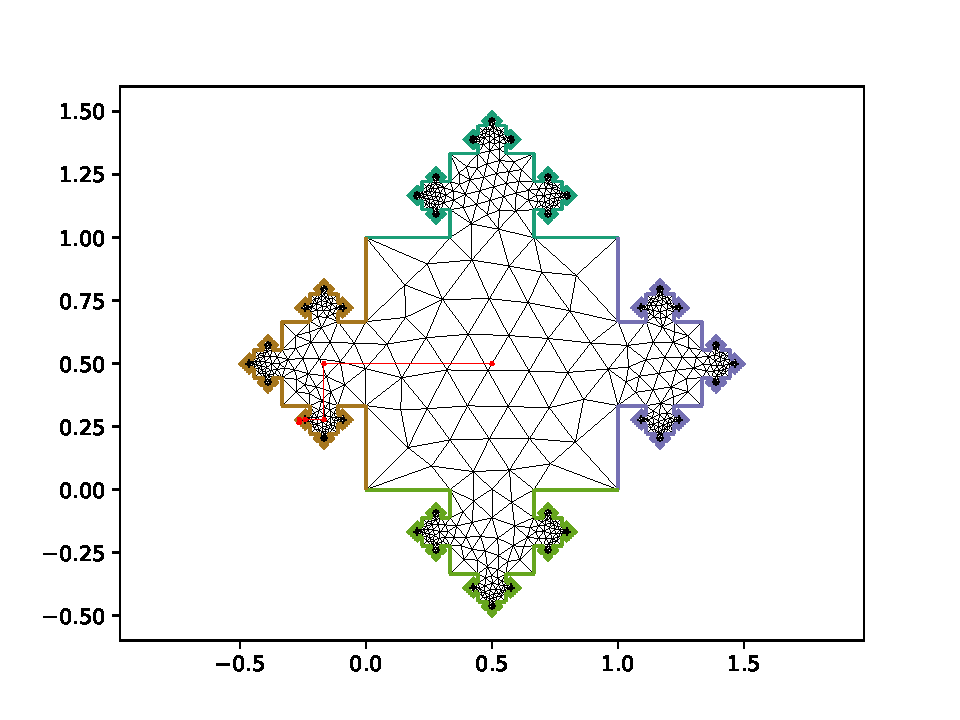
\includegraphics[width=\linewidth]{figures/Ex3/path_8_trial_0.pdf}
\end{subfigure}
 \begin{subfigure}[h]{0.45\linewidth}
    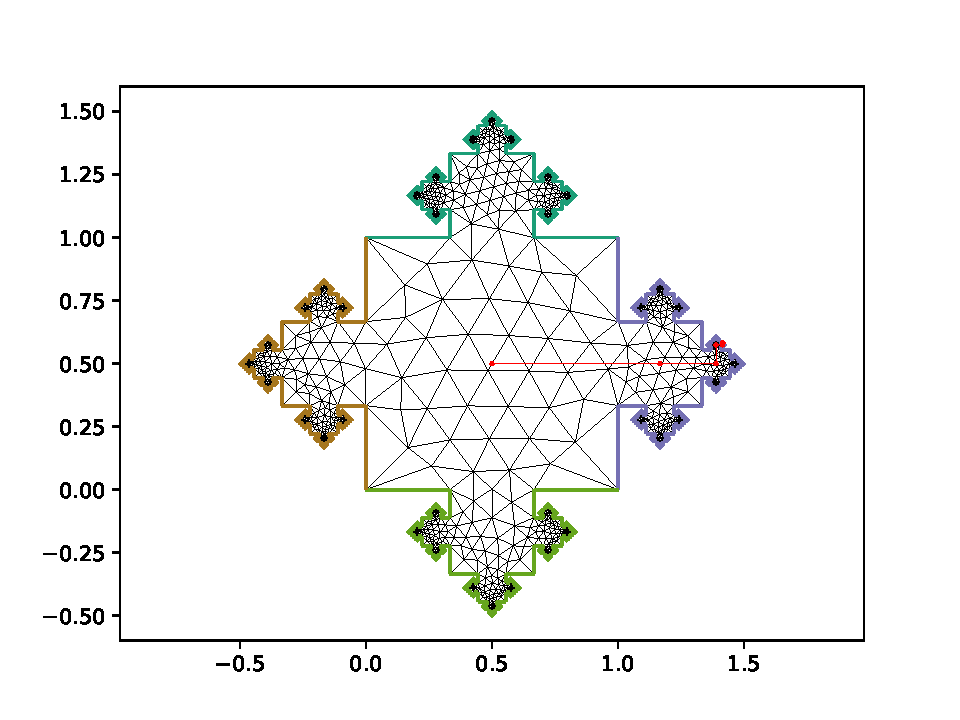
\includegraphics[width=\linewidth]{figures/Ex3/path_8_trial_1.pdf}
\end{subfigure}
  \caption{ Two random path on the unit square with $8$ snowflake iterations. }
 \end{figure}
Let $dx_i=(1/3)^i$. Then we would like to approximate $u(\textbf{x}_i)$ as a function of $dx_i$ in the form 
$$
u(\textbf{x}_i)=c(dx_i)^{\alpha}
$$
By taking the log on both ends, 
$$
\log u(\textbf{x}_i)=\log c+\alpha\log(dx_i),\quad 0\leq i\leq n.
$$
The coefficients $c$ and $\alpha$  are found by least squares approximation.  

After running 500 random path, we get:
\begin{table}[H]
\centering
\begin{tabular}{|c|c|c|}
              &  Mean & Standard deviation  \\ \hline
 $c$        &0.047939  & 0.0053037    \\
  $\alpha$& 2.1734 & 0.095348  
\end{tabular}
\end{table}

  \begin{figure}[H]%
    \centering
         \begin{subfigure}[h]{0.45\linewidth}
         \caption{$c=0.051$, $\alpha=2.03708$}
\includegraphics[width=\linewidth]{figures/Ex3/evaluate_8_trial_1.png}
\end{subfigure}
 \begin{subfigure}[h]{0.45\linewidth}
         \caption{$c=0.0519$, $\alpha=2.15278$}
\includegraphics[width=\linewidth]{figures/Ex3/evaluate_8_trial_2.png}
\end{subfigure}
  \caption{On unit square with $8$ snowflake iterations.  Result of different random path }
  \label{Ex3_evaluation}
 \end{figure}
 
 
 

   
\bibliographystyle{unsrt}
\bibliography{bibfile}
\end{document}
